% !TeX spellcheck = en_GB
%\documentclass[handout]{beamer}\mode<presentation>{\usetheme{AMSCesenaPurpleAndGold}}
\documentclass[presentation]{beamer}\mode<presentation>{\usetheme{AMSCesenaPurpleAndGold}}
%%%%

\usepackage{sd-lab-building-agents}
\usepackage{my-listings}
\usepackage{forloop}

\newcommand{\labN}{4}
\newcommand{\labGroup}{https://gitlab.com/pika-lab/courses/ds/ay2021}
\newcommand{\labRepo}{\labGroup/lab-\labN}


\title[L\labN{} -- Building Agents]{L\labN{} -- Building Agents from Scratch}
%
\subtitle[SD]{Distributed Systems / Technologies}
%
\author[Ciatto \and Omicini]
{\emph{Giovanni Ciatto} \and Andrea Omicini\\
	\texttt{giovanni.ciatto@unibo.it \and andrea.omicini@unibo.it}}
%
\institute[DISI, Univ. Bologna]
{Dipartimento di Informatica -- Scienza e Ingegneria (DISI)\\\textsc{Alma Mater Studiorum} -- Universit{\`a} di Bologna a Cesena}
%
\date[A.Y. 2020/2021]{Academic Year 2020/2021}

\setbeamercovered{transparent}

\AtBeginSection{
	\begin{frame}[c]\frametitle{Outline}
		% 		\begin{multicols}{2}
		\tableofcontents[sectionstyle=show/shaded, subsectionstyle=hide/hide, subsubsectionstyle=hide/hide]
		% 		\end{multicols}
	\end{frame}
}

\AtBeginSubsection{
	\begin{frame}[c]\frametitle{Next in Line\ldots}
		\begin{multicols}{2}
			\tableofcontents[sectionstyle=show/shaded, subsectionstyle=show/shaded, subsubsectionstyle=hide/hide]
		\end{multicols}
	\end{frame}
}

\begin{document}

%\\\\\\\\\\\\\\\\\\\\\
\frame{\titlepage}
%\\\\\\\\\\\\\\\\\\\\\

\section{Motivation \& Lecture Goals}

\begin{frame}[allowframebreaks]
\frametitle{Motivation \& Lecture Goals}

	\begin{itemize}
		\item This lecture is aimed at showing how \jade{}-like agents can be constructed from scratch
		%
		\begin{itemize}
			\item we will build a simple framework for MAS execution $\ldots$
			\item $\ldots$ to be extended in future lectures with interaction- and distribution-related features
		\end{itemize}

		\bigskip

		\item Building an agent framework requires defining, at least:
		%
		\begin{enumerate}
			\item how agents are executed, created, stopped, or paused (and therefore resumed)
			\item how agents may carry on several \emph{behaviours}, concurrently
			\item how agents may \emph{interact}, possibly in spite of distribution
		\end{enumerate}
	\end{itemize}

\end{frame}

\subsection{About the practical activities}

\begin{frame}
\frametitle{Lab \labN{} Repository on GitLab}

	\begin{itemize}
		\item Examples and exercises described in this lecture are provided by means of the following GitLab repository:
		%
		\begin{center}
			\url{\labRepo}
		\end{center}

		\vfill

		\item Clone it on your machine using Git
		%
		\begin{itemize}
		    \item[\$] \texttt{git clone \textit{<repo URL>}}
		\end{itemize}

		\vfill

		\item Even if a minimal environment simply relying on a text editor + Gradle is sufficient for this lab, we kindly suggest to import the cloned repository into some IDE, e.g. IntelliJ Idea or Eclipse
		%
		%
		\begin{itemize}
		    \item in case of problems in importing the project on IntelliJ, try to downgrade the gradle wrapper
		\end{itemize}

		\vfill

		\item In order to be able to submit your exercises, please ensure you requested access to the \href{\labGroup}{GitLab group of the course}
	\end{itemize}

\end{frame}

\section{Towards Multi-Agent Systems}

\subsection{Metamodel}

\begin{frame}[allowframebreaks]
\frametitle{Metamodel}

	\begin{block}{MAS}
	    We consider a MAS to be composed by a number of agents \alert{interacting} within an environment
	\end{block}

	\bigskip

	\begin{block}{Environment}
		We consider an Environment as a container of agents, exposing \emph{shared} facilities aimed at \alert{supporting} the agents' \alert{creation}, and \alert{interaction}
	\end{block}

	\bigskip

	\begin{block}{Agent}
	    We consider an Agent as a \alert{named} object (data + behaviour) coming with its own \alert{internal scheduler} aimed at executing an arbitrary amount of \alert{behaviours} concurrently
	\end{block}

	\bigskip

	\begin{block}{Agents' Finite State Machine (FSM)}
		We assume each Agent is moved by an internal FSM aimed supporting life-cycle management operations such as: \emph{start}, \emph{restart}, \emph{pause}, \emph{resume}, \emph{stop}
	\end{block}

	\bigskip

	\begin{block}{Agent Identifier (AID)}
		We assume each Agent is uniquely identified by an AID:
		%
		\begin{center}
			AID = agent name + environment name
		\end{center}
	\end{block}

	\bigskip

	\begin{block}{Behaviours}
		We consider a Behaviour as an atomic or composite action an agent may carry on, concurrently (w.r.t. other Behaviours)
	\end{block}

	\bigskip

	\begin{block}{Agents' Interaction}
		Any means letting an agent affect the operation of other agents.
		Can be achieved in several ways (message-passing, shared-memory, stigmergy, etc).
		%
		\begin{center}\bfseries
			(we will endow agents with interaction in future lectures, via \linda{})
		\end{center}
	\end{block}

\end{frame}

\subsection{Activity Overview}

\begin{frame}%[allowframebreaks]
	\frametitle{Activity Overview}

	For each notion in the aforementioned meta-model, we will:
	%
	\vfill
	%
	\begin{enumerate}
		\item draw the general design

		\vfill

		\item propose a minimal Java interface

		\vfill

		\item sketch the architecture

		\vfill

		\item describe the implementation stub

		\vfill

		\item complete the implementation via exercises
	\end{enumerate}

\end{frame}

\subsection{Agent Identifiers}

\begin{frame}{\texttt{AID} Class}

	\lstinputlisting{code/AID.java}

\end{frame}

\begin{frame}{\texttt{AID} Class -- Design Rationale}

	\begin{itemize}

		\item In the general case, agents are identified by two names:
		%
		\begin{itemize}
			\item the agent's \alert{local} name
			\item the name of the environment hosting the agent
		\end{itemize}

		\vfill

		\item In some cases, the environment name maybe unknown, thus missing
		%
		\begin{itemize}
			\item in this case, we say the \texttt{AID} is \alert{local}
			\item otherwise, we say the \texttt{AID} is \alert{full}
		\end{itemize}

		\vfill

		\item Full \texttt{AID} can be created via the \texttt{AID.full} \alert{static} method

		\vfill

		\item Local \texttt{AID} can be created via the \texttt{AID.local} \alert{static} method

		\vfill

		\item The \texttt{AID.parse} \alert{static} method can be used to parse \texttt{AID} from well formed strings in the form: \texttt{"localName@environmentName"}
	\end{itemize}

\end{frame}

\subsection{Environment}

\begin{frame}[allowframebreaks]{Environment Interface}

    \lstinputlisting{code/Environment.java}

\end{frame}

\begin{frame}{\texttt{Environment} Interface -- Design Rationale}

    \begin{itemize}

    	\item Given some subtype \texttt{A} of \texttt{AgentFSM}, an environment can only host agents whose type is \texttt{A}
    	%
    	\begin{itemize}
    		\item the actual type \texttt{A} is specified at instantiation time
    	\end{itemize}

	    \vfill

	    \item Environments have their own unique name

    	\vfill

    	\item The set of \texttt{AID} currently hosted by the environment can be retrieved via the \alert{\texttt{getAgents}} method

    	\vfill

        \item Via environments, agents' FSM can either
        %
        \begin{itemize}
            \item be created outside the environment and then join it via the \alert{\texttt{register}} method
            %
            \item be created as part of the environment, via the \alert{\texttt{create}} method
        \end{itemize}

    	\vfill

    	\item Users can block until all agents terminated via the \alert{\texttt{awaitAllAgents}} method

    \end{itemize}

\end{frame}

\begin{frame}[allowframebreaks]{\texttt{Environment} Interface -- Implementations}

    \begin{block}{\texttt{sd.lab.agency.impl.\textit{AbstractEnvironment}}}
        Provides common facilities for agents' initialisation and registration, which can be reused by sub-classes
    \end{block}

    \bigskip

    \begin{exampleblock}{\texttt{sd.lab.agency.impl.\textit{MultiThreadedEnvironment}}}
        \begin{itemize}
			\item A particular sort of environment where each agent is executed on its own thread
			\item Instances of \texttt{MultiThreadedEnvironment} can be instantiated via the \alert{\texttt{Environment.multiThreaded}} static method
			\item This will be implemented and used in exercise \labN{}-1
        \end{itemize}
    \end{exampleblock}

	\bigskip

	\begin{exampleblock}{\texttt{sd.lab.agency.impl.\textit{ExecutorBasedEnvironment}}}
		\begin{itemize}
			\item A particular sort of environment where all agents are executed on the same executor service
			\item Instances of \texttt{ExecutorBasedEnvironment} can be instantiated via the \alert{\texttt{Environment.executorBased}} static method
			\item This will be implemented and used in exercise \labN{}-2 (which is \emph{optional})
		\end{itemize}
	\end{exampleblock}

    \bigskip

    \begin{itemize}
        \item[!] these classes are already implemented
    \end{itemize}

    \framebreak

    \begin{alertblock}{(Spoiler Alert) \textbf{Distributed} Environment}
        \begin{itemize}
        	\item Supports the interaction among agents running on different machines
        	\item Will be designed and implemented in future lectures
        \end{itemize}
    \end{alertblock}

\end{frame}


\subsection{Agent FSM}

\begin{frame}[allowframebreaks]{\texttt{AgentFSM} Interface}

    \lstinputlisting{code/AgentFSM.java}

\end{frame}

\begin{frame}[allowframebreaks]{\texttt{AgentFSM} Interface -- Rationale}

    % \begin{block}{Agent VS User perspectives}
    %     The functioning of agents can be described and understood according to two different perspectives:

    % \end{block}

    Expected functioning of all objects of type \alert{\texttt{AgentFSM}}:
    %
    \bigskip
    %
    \begin{itemize}
        \item an FSM is created by some other entity as an ordinary Java object

        \bigskip

        \item it may be started from outside by means of the \texttt{\alert{start()}} method

        \bigskip

        \item once started, the following things should happen:
        %
        \begin{enumerate}
            \item the \texttt{\alert{onBegin()}} callback is executed \alert{just once}

            \item \alert{after} that, the \texttt{\alert{onRun()}} method is executed an \alert{unlimited} amount of times, sequentially

            \item the sequence of executions of \texttt{onRun()} can only be interrupted by the agent itself by calling the \texttt{\alert{stop()}} method inside its \texttt{onBegin()} or \texttt{onRun()} callbacks
        \end{enumerate}

        \framebreak

        % \item if the agent calls its \texttt{Agent::\alert{pause()}} method, the sequence of \texttt{onRun()} is interrupted as well

        % \vspace{.5cm}

        % \item however, if some external entity calls the
        % \texttt{Agent::\alert{resume()}} method on a paused agents, the sequence of \texttt{onRun()} is resumed \alert{from where it had been interrupted}

        % \vspace{.5cm}

        % \item if the agent calls its \texttt{Agent::\alert{restart()}} method, the sequence of \texttt{onRun()} is restarted---and the \texttt{onBegin()} method is executed one more time

        % \vspace{.5cm}

        % \item finally, external entities can wait for an agent's termination by means of the \texttt{Agent::\alert{await()}} method and its overloads

        % \framebreak

        % \item in any scenario, if some \alert{uncaught exception} is thrown within the \texttt{onBegin()} or \texttt{onRun()} methods, the \texttt{Agent::\alert{onUncaughtError(Exception)}} callback is called

        % \vspace{.5cm}

        % \item what happens next depends on the value returned by the \texttt{onUncaughtError(Exception)} callback, which is of type \alert{\texttt{AndThen}}
        % %
        % \begin{description}
        %     \item[\texttt{CONTINUE}] | the exception is ignored and the sequence of \texttt{onRun()} is unaffected

        %     \item[\texttt{PAUSE}] | the sequence of \texttt{onRun()} is paused
        % \end{description}

        \item after that, the agent \alert{terminates}---which means that all entities which possibly invoked the \texttt{\alert{await()}} method, can now resume their computation

        \bigskip

        \item within its \texttt{onBegin()}, \texttt{onRun()}, or \texttt{onEnd()} methods, an agent can call the following methods affecting its own control flow and, in particular, the sequence of \texttt{on*()} methods executions:
        %
        \begin{description}\small
            \item[\texttt{stop()}] states that the next method to be executed should be \texttt{onEnd()}

            \item[\texttt{restart()}] states that the next method to be executed should be \texttt{onBegin()}

            \item[\texttt{pause()}] states that no method should be executed next, until \texttt{resume()} is called

            \item[\texttt{resume()}] states that the sequence of \texttt{on*()} methods executions should be resumed starting from where it was interrupted by the \texttt{pause()}
        \end{description}

        \framebreak

        \item \alert{no uncaught exception} should be able to break the aforementioned workflow

        \bigskip

        \item to this end, \texttt{\alert{onUncaughtError(Exception)}} callback is executed for each exception which is not caught within the \texttt{onBegin()}, \texttt{onRun()}, or \texttt{onEnd()} methods

        \bigskip

        \item after the \texttt{onUncaughtError(Exception)} callback is executed, the aforementioned workflow continues as if the exception didn't occurred (i.e. the series of \texttt{onRun()} is resumed)
        %
        \begin{itemize}
            \item unless the agent calls some life-cycle control method within the \texttt{onUncaughtError(Exception)} callback
        \end{itemize}
    \end{itemize}
\end{frame}

\begin{frame}{External VS internal API}

\begin{itemize}
    \item \texttt{AgentFSM} is actually the union of two API targetting different usages

    \vfill

    \item The \alert{external} API comprehends methods which are to be called \alert{from outside} the agent
    %
    \begin{itemize}
        \item[eg] method \texttt{\alert{start()}}
        \item[eg] method \texttt{\alert{await()}}
        \item[eg] method \texttt{\alert{resume()}}
    \end{itemize}

    \vfill

    \item The \alert{internal} API comprehends methods which are to be called \alert{from within} the agent itself
    %
    \begin{itemize}
        \item[eg] method \texttt{\alert{stop()}}
        \item[eg] method \texttt{\alert{pause()}}
        \item[eg] method \texttt{\alert{pause()}}
        \item[eg] method \texttt{\alert{restart()}}
    \end{itemize}

    \vfill

    \item Briefly speking, methods composing the \alert{internal} API can be called by agent implementors, \alert{only} within the \texttt{on*()} callbacks
    %
    \begin{itemize}
        \item calling them elsewhere may lead to unexpected \& unpredicatable behaviour
    \end{itemize}
\end{itemize}

\end{frame}

\subsubsection{Examples of valid scenarios}

\begin{frame}{Normal Flow}\centering
    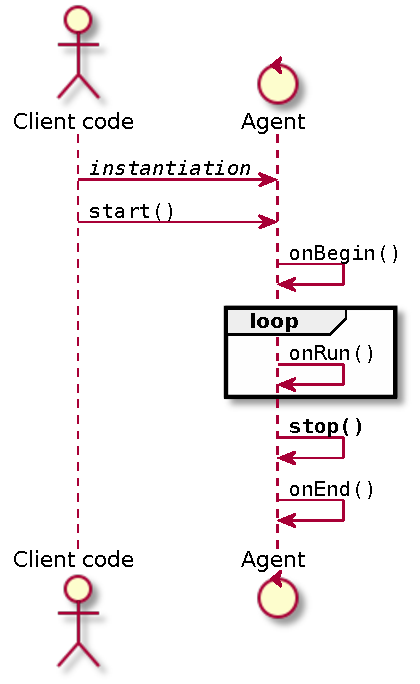
\includegraphics[height=.8\textheight]{img/normal-flow.pdf}
\end{frame}

\begin{frame}{Pause and Resume}\centering
    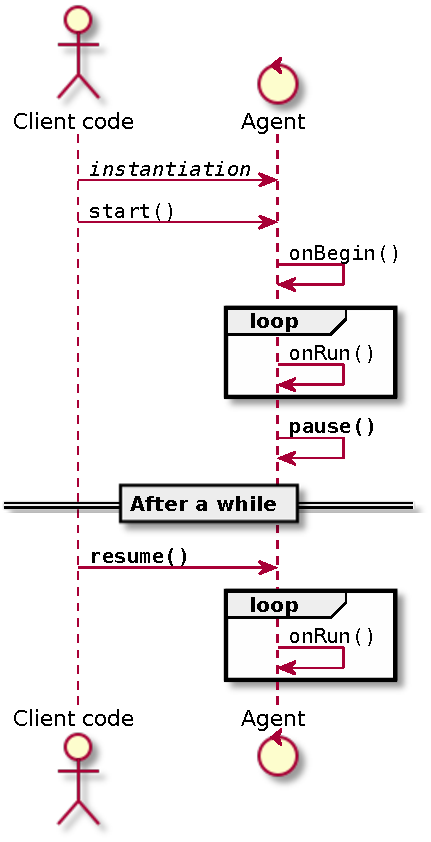
\includegraphics[height=.8\textheight]{img/paused-flow.pdf}
\end{frame}

\begin{frame}{Restart}\centering
	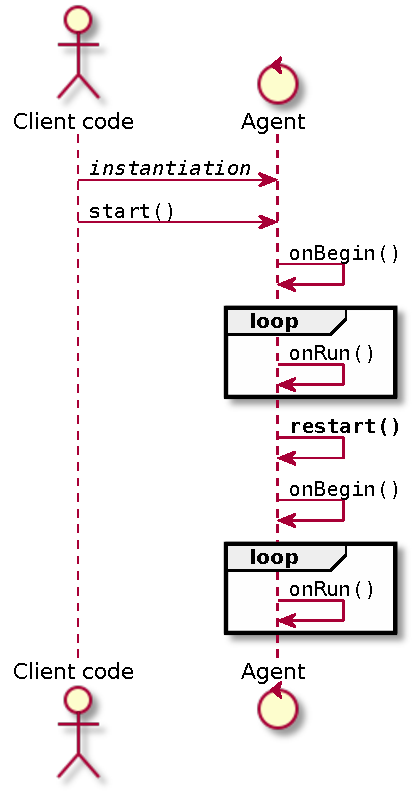
\includegraphics[height=.8\textheight]{img/restarted-flow.pdf}
\end{frame}

\begin{frame}[allowframebreaks]{Uncaught Exceptions}
    \begin{center}
    	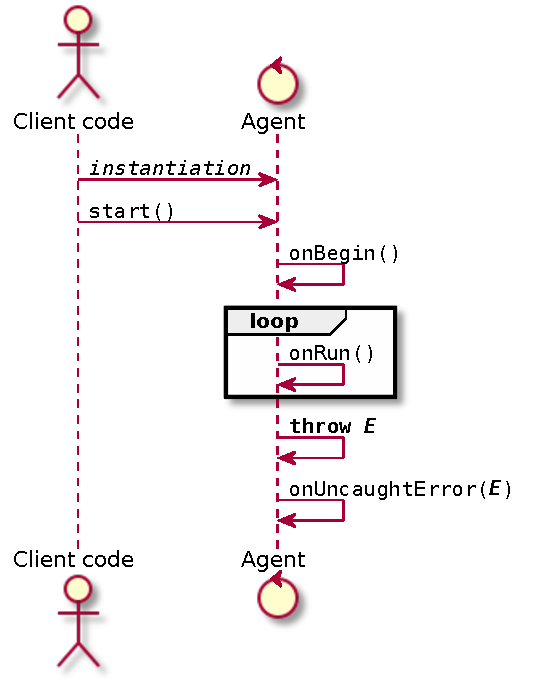
\includegraphics[height=.8\textheight]{img/exceptional-flow-1.pdf}
    \end{center}

    \begin{center}
    	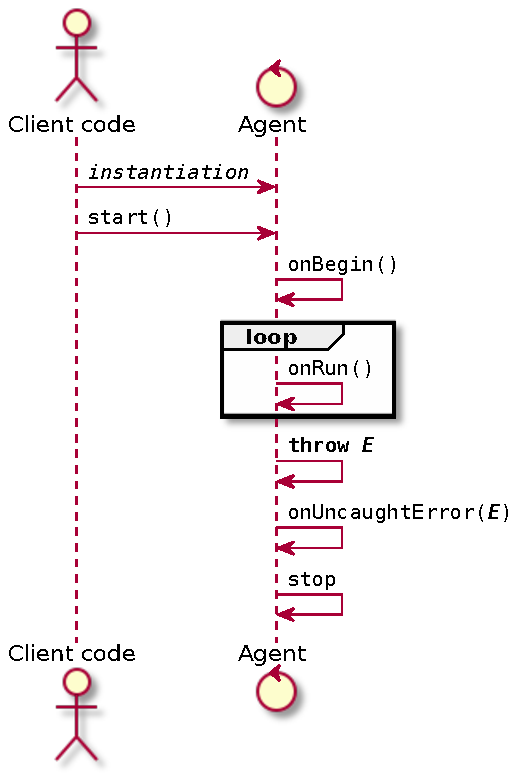
\includegraphics[height=.8\textheight]{img/exceptional-flow-2.pdf}
    \end{center}

    \begin{center}
    	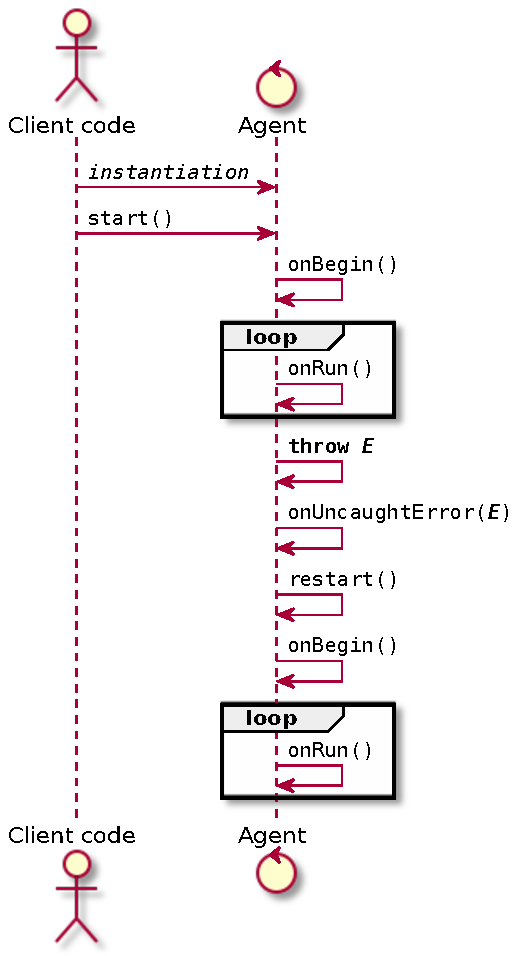
\includegraphics[height=.8\textheight]{img/exceptional-flow-3.pdf}
    \end{center}
\end{frame}

\subsubsection{Usage Example}

\begin{frame}[allowframebreaks]{Example}
    Setting up the environment:
    %
    \lstinputlisting{code/ExampleEnvironment.java}

    \framebreak

    The agent FSM:
    %
    \lstinputlisting{code/ExampleAgentFSM.java}

    Expected logs:
    %
    \begin{itemize}
    	\item[$\rightarrow$] 0, 1, 2, 3, 4, 5, 6
    \end{itemize}
\end{frame}

\begin{frame}[allowframebreaks]{Agent FSM state diagram}

    \begin{itemize}
        \item The agents' functioning just described can be modelled through a state diagram

        \bigskip

        \item In any given moment, the FSM may be in any of $5+1$ states:
        %
        \begin{description}
            \item[\texttt{CREATED}] | the agent has been instantiated but not yet started

            \item[\texttt{STARTED}] | after the \texttt{start()} method has been called

            \item[\texttt{RUNNING}] | after the \texttt{onBegin()} callback has been executed

            \item[\texttt{PAUSED}] | after the \texttt{pause()} method has been called

            \item[\texttt{STOPPED}] | after the \texttt{stop()} method has been called

            \item[terminated] | after the \texttt{onEnd()} callback has been executed
        \end{description}

    	\bigskip

    	\item Such states are represented by the \texttt{sd.lab.agency.fsm.impl.\alert{State}} enum

        \framebreak

        \item State transition are usually provoked by invocations of the \alert{control methods}
        %
        \begin{itemize}
        	\item i.e., the \texttt{start()}, \texttt{stop()}, \texttt{restart()}, \texttt{pause()}, or \texttt{resume()} methods
        \end{itemize}

%    	\bigskip

%        \item Such methods feed the FSM with values of type \texttt{sd.lab.agency.fsm.impl.\alert{Command}}
%        %
%        \begin{itemize}
%        	\item i.e., \texttt{CONTINUE}, \texttt{RESTART}, \texttt{PAUSE}, or \texttt{STOP}
%        	\item if no control method is called within a callback, \texttt{\alert{CONTINUE}} is fed to the FSM, by default
%        \end{itemize}

        \bigskip

        \item State transition of the FSM provoke the invocation of callbacks
         %
        \begin{itemize}
        	\item i.e., \texttt{onBegin()}, \texttt{onRun()}, \texttt{onEnd()}, or \texttt{onUncaughtError(...)}
        \end{itemize}
    \end{itemize}

    \framebreak

    \begin{center}
%        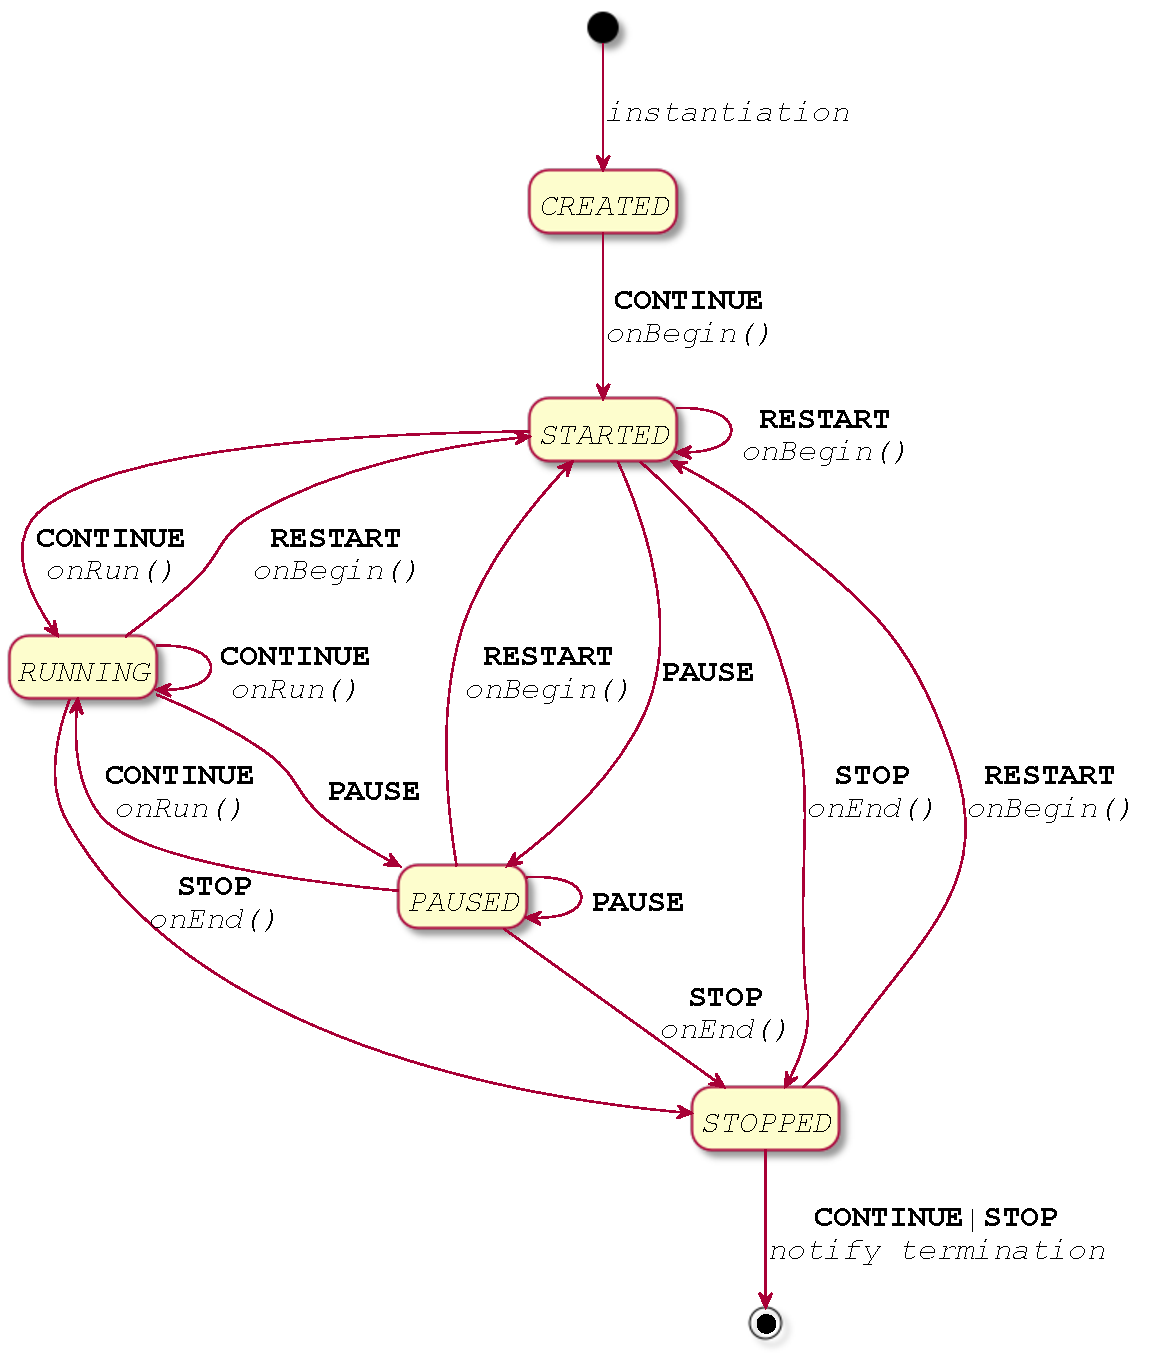
\includegraphics[height=.9\textheight]{img/fsa.pdf}
        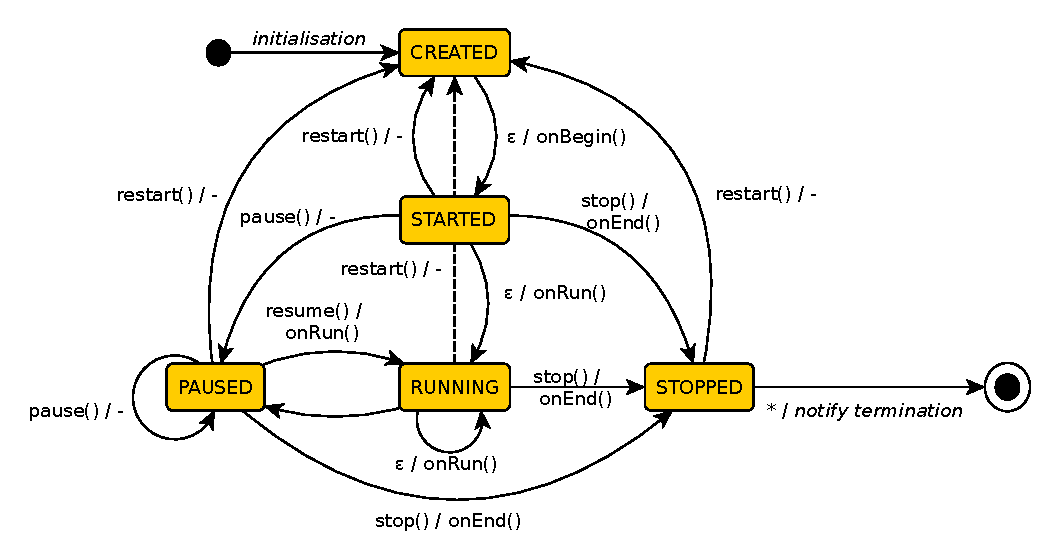
\includegraphics[width=.8\linewidth]{img/fsm.pdf}
    \end{center}

    \begin{block}{Legend}\centering
        life-cycle method $(input)$ / callback $(output)$
    \end{block}

\end{frame}

\section{Exercises (pt. 1)}

\startExercise

\subsection{Thread-based agent FSM}

\begin{frame}[c, allowframebreaks]
    \frametitle{Exercise \currentExercise{} -- Thread-based agent FSM}

    \begin{block}{GitLab repository}\centering
        \url{\labRepo}
    \end{block}

    \bigskip

    Consider the class stub \texttt{sd.lab.agency.fsm.impl.\alert{ThreadBasedAgentFSM}}:
    %
    \bigskip
    %
    \begin{itemize}
        \item It implements the agent FSM by leveraging a thread for each agent

        \framebreak

        \item Intuitively and agent FSM's thread works as follows:
        %
        \lstinputlisting[language=Java]{code/SimplifiedFSMThread.java}

        \item However, this solution comes with several drawbacks:
        %
        \begin{itemize}
            \item is the expected callbacks workflow \emph{always} respected?
            \item how can the methods \texttt{pause}, \texttt{resume}, \texttt{restart}, and \texttt{await} be implemented?
        \end{itemize}

    \end{itemize}

    \framebreak

    Expected activity:
    %
    \bigskip
    %
    \begin{enumerate}

        \item Complete the implementation of the \texttt{ThreadBasedAgentFSM} class\ldots

        \bigskip

        \item \ldots in such a way that tests in \texttt{sd.lab.agency.\alert{TestThreadedAgentFSM}} are all satisfied

        \bigskip

        \item Submit your exercise to the following branch on Lab \labN{} repository
        %
        \begin{center}
            \texttt{submissions/\textit{name.surname}}
        \end{center}

        \bigskip

        \item Continuous Integration will automatically run tests
    \end{enumerate}

\end{frame}

\startExercise

\subsection{Executor-Service-based agent FSM (Advanced)}

\begin{frame}[c, allowframebreaks]
    \frametitle{Exercise \currentExercise{} -- Executor-Service-based agent FSM}

    \begin{alertblock}{This is an \textbf{advanced} exercise}
        \begin{itemize}
            \item feel free to skip it
            \item try it if you are curious about the idea of making MAS scalable
        \end{itemize}
    \end{alertblock}

    \bigskip

    \begin{block}{Motivation}
        \begin{itemize}
            \item the 1-agent-1-thread approach makes MAS poorly scalable
            %
            \begin{itemize}
                \item threads are resource greedy and slow upon startup
            \end{itemize}

            \item the 1-mas-1-executor-service approach if more flexible
            %
            \begin{itemize}
                \item agents \emph{share} the same executor service, \emph{hosted by the environment}
                \item the executor service takes care of spawning threads \emph{upon need}
                \item the MAS as a whole is more resource efficient
            \end{itemize}
        \end{itemize}
    \end{block}

    \bigskip

    Consider the class stub \texttt{sd.lab.agency.fsm.impl.\alert{ExecutorBasedAgentFSM}}:
    %
    \bigskip
    %
    \begin{itemize}
        \item It implements the agent FSM by leveraging on a shared executor service
        %
        \begin{itemize}
            \item which is supposed to be provided by the environment$\ldots$
            \item $\ldots$ upon agent's creation or registration
        \end{itemize}
    \end{itemize}

    \framebreak

    Expected activity:
    %
    \bigskip
    %
    \begin{enumerate}

        \item Complete the implementation of the \texttt{ExecutorBasedAgentFSM} class\ldots

        \bigskip

        \item \ldots in such a way that tests in \texttt{sd.lab.agency.\alert{TestExecutorAgentFSM}} are all satisfied

        \bigskip

        \item You will deeply leverage \& practice with \emph{asynchronous programming}

        \bigskip

        \item Submit your exercise to the following branch on Lab \labN{} repository
        %
        \begin{center}
            \texttt{submissions/\textit{name.surname}}
        \end{center}

        \bigskip

        \item Continuous Integration will automatically run tests
    \end{enumerate}

\end{frame}

\section{Towards Agents with Behaviours}

\subsection{The notion of \texttt{Agent}}

\begin{frame}[allowframebreaks]
    \frametitle{The \texttt{Agent} interface}

    \begin{itemize}
        \item To increase our \emph{level of abstraction} we introduce a novel notion of \alert{\texttt{Agent}}
        %
        \begin{itemize}
            \item which borrows JADE's notion of \texttt{\alert{Behaviour}}
        \end{itemize}
    \end{itemize}

    \bigskip

    \lstinputlisting{code/Agent.java}

    \framebreak

    \begin{itemize}
        \item An \texttt{Agent} is a particular sort of \texttt{AgentFSM}

        \bigskip

        \item However, \texttt{Agent}s expose a \alert{queue} of \alert{behaviours} which they will eventually execute
        %
        \begin{itemize}
            \item conventionally, we call it ``the \alert{to-do list}''
        \end{itemize}

        \bigskip

        \item Each \texttt{Agent} comes equipped with an \alert{internal scheduler} supporting the execution of a number of \texttt{Behaviour}s
        %
        \begin{itemize}
            \item so, their \texttt{on*()} callbacks must not be overridden by agents' users

        \end{itemize}

        \bigskip

        \item Behaviours may be added within the \alert{\texttt{setup()}} callback or dynamically, i.e. while executing other behaviours

        \bigskip

        \item Articulated behaviours are build through \alert{composition} of simpler behaviours

    \end{itemize}

\end{frame}

\begin{frame}%[allowframebreaks]
    \frametitle{\texttt{Agent} -- Usage Example}
    \lstinputlisting{code/DoubleCounter.java}

    \vfill

    \begin{itemize}
        \item The agent is carrying on two \alert{concurrent activities}, called \emph{behaviours}
        %
        \begin{itemize}
            \item in particular, a counter is increased and another is decreased until they meet halfway
        \end{itemize}

        \vfill

        \item A behaviour is any instance of the \texttt{\alert{Behaviour}} type
    \end{itemize}

\end{frame}

\subsection{The notion of \texttt{Behaviour}}

\begin{frame}%[allowframebreaks]
    \frametitle{The \texttt{{\small{}sd.lab.agency.behaviour.}Behaviour} interface}

    \lstinputlisting{code/Behaviour.java}

\end{frame}

\begin{frame}%[allowframebreaks]
    \frametitle{\texttt{Behaviour} interface -- Expected functioning}

    \begin{itemize}
        \item Agents of type \texttt{Agent} can dynamically \alert{schedule \& execute} behaviours thanks to an \alert{internal scheduler}

        \vfill

        \item A \texttt{Behaviour} may scheduled several times, and every time its \alert{\texttt{execute(\ldots)}} method is run
        %
        \begin{itemize}
            \item unless it is \alert{paused}, i.e, if its \texttt{\alert{isPaused()}} methods returns true
        \end{itemize}

        \vfill

        \item Each agent takes care of passing a reference to itself to the \texttt{\alert{execute(\ldots)}} method of each behaviour it executes

        \vfill

        \item If, after its execution, the behaviour is over, i.e. if its \texttt{\alert{isOver()}} returns true, the agent's scheduler simply drops it

        \vfill

        \item By default, behaviours are executed (at least) once and they are not paused
    \end{itemize}

\end{frame}

\begin{frame}%[allowframebreaks]
    \frametitle{About \texttt{Behaviour}s}

    \begin{itemize}
        \item \texttt{Behaviour}s can either \alert{atomic} or \alert{composed} by other sub-behaviours
        %
        \begin{itemize}
            \item \alert{Composed} behaviours perform some sort of \alert{internal scheduling} within their \texttt{execute(\ldots)} method, atomic behaviours do not
        \end{itemize}

        \vfill

        \item \texttt{Behaviour}s can either \alert{state\emph{less}} or \alert{state\emph{ful}} (a.k.a. immutable or mutable)
        %
        \begin{itemize}
            \item A state\emph{less} behaviour can be \alert{re-executed \& re-used} several times

            \item A state\emph{ful} behaviour can only be executed \alert{once} and must be \alert{deep-cloned} before in order for the copy to be executable again
            %
            \begin{itemize}
                \item this is why we need the \texttt{Behaviour.\alert{deepClone()}} method
            \end{itemize}
        \end{itemize}

        \vfill

        \item The \texttt{Behaviour} interface also exposes some \alert{static methods} letting you instantiate standard behaviours by means of a compact notation

        \vfill

        \item The \texttt{Behaviour} interface also exposes some \alert{default methods} letting you combine behaviours into complex ones by means of a \alert{fluent} notation
    \end{itemize}

\end{frame}

\begin{frame}[allowframebreaks]
    \frametitle{\texttt{Behaviour} interface -- Creating behaviours}

    Behaviours can be instantiated by means of the many \alert{static} methods:
    %
    \bigskip
    %
    \begin{description}
        \item[\texttt{{\small{}Behaviour.}of(\textit{lambdaExpression})}] creates a \alert{one-shot} behaviour which will eventually execute \texttt{\textit{lambdaExpression}}
        %
        \begin{itemize}\small
            \item the behaviour terminates only after \texttt{\textit{lambdaExpression}} has been executed
            \item the behaviour cannot be paused
        \end{itemize}

        \bigskip

        \item[\texttt{{\small{}Behaviour.}sequence(\textit{b1}, \ldots, \textit{bN})}] creates a \alert{sequential} behaviour that executes sub-behaviours \texttt{\textit{b1}}, \ldots, \texttt{\textit{bN}} \alert{in a row}
        %
        \begin{itemize}\small
            \item the behaviour terminates after \alert{all} sub-behaviours are over
            \item the behaviour is paused if the next sub-behaviour to execute is paused
            \item sub-behaviour \texttt{\textit{b$_i$}} is \alert{not} executed until \texttt{\textit{b$_{i-1}$}} is over
        \end{itemize}

        \bigskip

        \item[\texttt{{\small{}Behaviour.}anyOf(\textit{b1}, \ldots, \textit{bN})}] creates a compound behaviour that executes sub-behaviours \texttt{\textit{b1}}, \ldots, \texttt{\textit{bN}} \alert{concurrently}
        %
        \begin{itemize}\small
            \item the behaviour terminates if \alert{at least} one \texttt{\textit{b$_i$}} is over
            \item the behaviour is paused if all sub-behaviours are paused
            \item the execution of sub-behaviours is interleaved
        \end{itemize}

        \vspace{.20cm}

        \item[\texttt{{\small{}Behaviour.}allOf(\textit{b1}, \ldots, \textit{bN})}] creates a compound behaviour that executes sub-behaviours \texttt{\textit{b1}}, \ldots, \texttt{\textit{bN}} \alert{concurrently}
        %
        \begin{itemize}\small
            \item the behaviour terminates if \alert{all} sub-behaviours over
            \item the behaviour is paused if all sub-behaviours are paused
            \item the execution of sub-behaviours is interleaved
        \end{itemize}

        \vspace{.20cm}

        \item[\texttt{{\small{}Behaviour.}wait(\textit{amountOfTime})}] creates an atomic behaviour that waits for an  \texttt{\textit{amountOfTime}}
        %
        \begin{itemize}\small
            \item the behaviour terminates after an \texttt{\textit{amountOfTime}} is elapsed since its first scheduling
            \item the behaviour cannot be paused
        \end{itemize}

%        \framebreak
%
%        \item[\texttt{{\small{}Behaviour.}lindaOperation(\textit{tsName}, \textit{invokeLambda}, \textit{callback})}] creates a behaviour which executes a \linda{} operation on some tuple space of choice, given its name
%        %
%        \begin{itemize}\small
%            \item the behaviour terminates after the \linda{} operation has been completed and the \texttt{\textit{callback}} has been executed
%            \item the behaviour is paused automatically while the operation is suspended
%        \end{itemize}
%
%        \framebreak
%
%        \item[\texttt{{\small{}Behaviour.}send(\textit{recipientID}, \textit{message}, \textit{callback})}] creates a behaviour which sends a \texttt{\textit{message}} to the agent identified by \texttt{\textit{recipientID}}
%        %
%        \begin{itemize}\small
%            \item the behaviour terminates after the message has been \alert{dispatched} and the \texttt{\textit{callback}} has been executed
%            \item the behaviour is paused automatically while the message is in transit
%        \end{itemize}
%
%        \bigskip
%
%        \item[\texttt{{\small{}Behaviour.}receive(\textit{callback})}] creates a behaviour which waits for a message directed towards the agent executing it
%        %
%        \begin{itemize}\small
%            \item the behaviour terminates after a message has been \alert{received} and the \texttt{\textit{callback}} has been executed
%            \item the behaviour is paused automatically until a message is received
%        \end{itemize}
    \end{description}

\end{frame}

\begin{frame}[allowframebreaks]
    \frametitle{\texttt{Behaviour} interface -- Combining behaviours}

    Behaviours can be combined by means of many \alert{default} methods:
    %
    \bigskip
    %
    \begin{description}
        \item[\texttt{\textit{b1}.andThen(\textit{b2}, \ldots, \textit{bN})}] is a shortcut for
        %
        \begin{center}
            \texttt{Behaviour.sequence(\textit{b1}, \textit{b2}, \ldots, \textit{bN})}
        \end{center}

        \bigskip

        \item[\texttt{\textit{b}.addTo(\textit{agent})}] is a shortcut for
        %
        \begin{center}
            \texttt{\textit{agent}.addBehaviour(\textit{b})}
        \end{center}

        \bigskip

        \item[\texttt{\textit{b}.removeFrom(\textit{agent})}] is a shortcut for
        %
        \begin{center}
            \texttt{\textit{agent}.removeBehaviour(\textit{b})}
        \end{center}

        \framebreak

        \item[\texttt{\textit{b}.repeatWhile(() -> \textit{condition})}] creates a compound behaviour where
        \texttt{\textit{b}} is repeated over and over again until \texttt{\textit{condition}} becomes false

        \bigskip

        \item[\texttt{\textit{b}.repeatUntil(() -> \textit{condition})}] creates a compound behaviour where
        \texttt{\textit{b}} is repeated over and over again until \texttt{\textit{condition}} becomes true

        \bigskip

        \item[\texttt{\textit{b}.repeatForEver()}] creates a compound behaviour where
        \texttt{\textit{b}} is repeated over and over again, indefinitely
    \end{description}
\end{frame}

\subsubsection{Usage Examples}

\begin{frame}%[allowframebreaks]
    \frametitle{Sequential behaviours}

    The following agents expose the same sequential behaviour:

    \vfill

    \begin{columns}
        \begin{column}{.48\linewidth}
            \lstinputlisting[basicstyle=\tiny\ttfamily]{code/sequence-example.java}
        \end{column}
        %	\vfill
        \begin{column}{.48\linewidth}
            \lstinputlisting[basicstyle=\tiny\ttfamily]{code/sequence-example-2.java}
        \end{column}
    \end{columns}

    \vfill

    Output:
    %
    \begin{itemize}
        \item \texttt{a, b, c}
    \end{itemize}

\end{frame}

\begin{frame}%[allowframebreaks]
    \frametitle{Parallel behaviours}

    The following agents employ different sorts of parallel behaviours:

    \vfill

    \begin{columns}
        \begin{column}{.48\linewidth}
            \lstinputlisting[basicstyle=\tiny\ttfamily]{code/any-example.java}

            \vspace{1cm}

            Output:
            %
            \begin{itemize}
                \item \texttt{1, a, 2, b, c}
            \end{itemize}
        \end{column}
        %	\vfill
        \begin{column}{.48\linewidth}
            \lstinputlisting[basicstyle=\tiny\ttfamily]{code/all-example.java}

            \vspace{1cm}

            Output:
            %
            \begin{itemize}
                \item \texttt{1, a, 2}
            \end{itemize}
        \end{column}
    \end{columns}

\end{frame}

\begin{frame}%[allowframebreaks]
    \frametitle{Do-While/Until behaviours}

    The following agents expose the same cyclic behaviour:

    \vfill

    \begin{columns}
        \begin{column}{.48\linewidth}
            \lstinputlisting[basicstyle=\tiny\ttfamily]{code/do-while-example.java}
        \end{column}
        %	\vfill
        \begin{column}{.48\linewidth}
            \lstinputlisting[basicstyle=\tiny\ttfamily]{code/do-until-example.java}
        \end{column}
    \end{columns}

    \vfill

    Output:
    %
    \begin{itemize}
        \item \texttt{0, 1, 2, 4, 5}
    \end{itemize}

\end{frame}

%\begin{frame}%[allowframebreaks]
%    \frametitle{Interacting with textual spaces}
%
%    The following agent performs a \linda{} operation on a tuple space named \texttt{\alert{inbox}}:
%
%    \vfill
%
%    \lstinputlisting{code/tuple-space-example.java}
%
%\end{frame}
%
%\begin{frame}%[allowframebreaks]
%    \frametitle{Send/Receive behaviours}
%
%    Agents may communicate directly through message passing:
%
%    \vfill
%
%    \begin{columns}
%        \begin{column}{.48\linewidth}
%            \lstinputlisting[basicstyle=\tiny\ttfamily]{code/sender-example.java}
%        \end{column}
%        %	\vfill
%        \begin{column}{.48\linewidth}
%            \lstinputlisting[basicstyle=\tiny\ttfamily]{code/receiver-example.java}
%        \end{column}
%    \end{columns}
%
%    \vfill
%
%    Output:
%    %
%    \begin{itemize}
%        \item \texttt{hello, world}
%    \end{itemize}
%
%\end{frame}

\begin{frame}
    \frametitle{Doing something for a while}

    \begin{block}{Design pattern}
        An OR-parallel behaviour composed by 2 sub-behaviours $B$ and $W$ -- where $W$ waits for some time $\Delta T$ -- means the agent will try to perform $B$ for no longer than $\Delta T$ units of time. After that $B$ will be interrupted.
    \end{block}

    \lstinputlisting{code/timed-op-example.java}

\end{frame}

\section{Exercises (pt. 2)}

\startExercise

\subsection{The \texttt{Agent}s' Internal Scheduler}

\begin{frame}[c, allowframebreaks]
    \frametitle{Exercise \currentExercise{} -- The \texttt{Agent}s' Internal Scheduler}

    Let's have a look to the \texttt{{\small{}sd.\allowbreak{}lab.\allowbreak{}agency.\allowbreak{}impl.\allowbreak{}}\alert{AbstractAgent}} class:
    %
    \lstinputlisting{code/AbstractAgent.java}

    \begin{exampleblock}{Abstract algorithm}
        \begin{enumerate}
            \item If the to-do list has no \alert{non-paused} behaviour, just pause the agent \emph{until some behaviour is added}

            \medskip

            \item Otherwise, let $b$ be the first non-paused behaviour in the queue

            \medskip

            \item Execute $b$

            \medskip

            \item If $b$ is over, just drop it

            \medskip

            \item Otherwise, re-insert $b$ to the end of the queue

            \medskip

            \item In any case, remove from the to-do-list any behaviour for which $b$ requested the removal
        \end{enumerate}
    \end{exampleblock}

    \begin{block}{Recall \jade{}'s theory}
        \begin{itemize}
            \item This is essentially a \alert{Round-Robin} scheduler

            \medskip

            \item where \alert{paused} behaviours are skipped

            \medskip

            \item where \alert{terminated} behaviours are dropped, and non-terminated ones are \alert{re-scheduled}
        \end{itemize}
    \end{block}

    \begin{alertblock}{\textbf{Subtle aspect}: Paused behaviour vs. Paused agent}
        \begin{itemize}
            \item Several behaviours may be paused

            \medskip

            \item However, the agent is \alert{paused} only if it runs out of non-paused behaviours

            \medskip

            \item This is why the agent must be resumed -- if paused -- whenever a new behaviour is added, or some behaviour is unpaused
            %
            \begin{itemize}
                \item this is the purpose of the \texttt{AgentFSM::\alert{resumeIfPaused}} method
            \end{itemize}
        \end{itemize}
    \end{alertblock}

    \framebreak

    Expected activity:
    %
    \bigskip
    %
    \begin{enumerate}

        \item Complete the implementation of the \texttt{AbstractAgent} class\ldots

        \bigskip

        \item \ldots in such a way that tests in \texttt{sd.lab.agency.behaviour.\alert{TestAgent}} are all satisfied
        %
        \begin{itemize}
            \item[!] notice that these tests won't pass until behaviours are implemented
            \item which is the aim of the next exercise
        \end{itemize}

        \bigskip

        \item Submit your exercise to the following branch on Lab \labN{} repository
        %
        \begin{center}
            \texttt{submissions/\textit{name.surname}}
        \end{center}

        \bigskip

        \item Continuous Integration will automatically run tests
    \end{enumerate}

\end{frame}

\startExercise

\subsection{Agents' \texttt{Behaviour}s}

\begin{frame}[c, allowframebreaks]
    \frametitle{Exercise \currentExercise{} -- Agents' \texttt{Behaviour}s}

    The implementations of standard behaviours are delegated to a number of classes in \texttt{sd.lab.agency.behaviour.impl.*}

    \begin{center}
        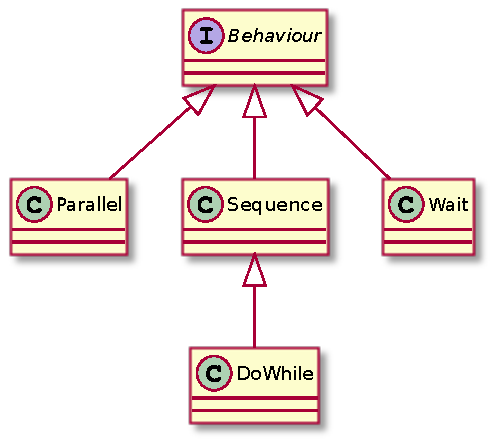
\includegraphics[width=.5\linewidth]{img/classes-overview.pdf}
    \end{center}
    %
    \hint{Detailed image by \href{http://www.plantuml.com/plantuml/svg/tLN1Rjim3BtxAmJqqc7h7mH3kmmxTKiG1-YPbhXK62rv4kLroFhlYnLNy1mvy8Bjqai2aq_cuoFzTEiP78UQ2cqOtLUGA3xW8xJQ1YVsXH1lnHugpmuaFulMQYNm2MLWl4uueBiT6XRG_RuPdwci9GGZj5z3yAYkpo1MBRgJ_82GGcoMP0qUGCz5yG8Hai1xSVS3D2-sxtlUiyb6e3KRz85u0lbER8Nh0F7CrP3UqjOD8KD5-2bmSDXHs26ldQsrFrywBqvUaRaot6kZODMW0zRMlEXnTHdFcUrgqzflk3BRSCYL3KYSrX6VE015aE24FwbJijDcrn7S9j0NgATvpfnvJh8DIjGjJWfrv19v_BDUBsvmnguE-0wsDft-ZDuVa7tNQl8rFKxKn_-SSYKQzTfboszbL2_hLrjqTVomu2TPK2U0qHXADFnN8pWgluO3bf3sPynXlWtcJIThK8b1YTy36ebvl_sFfXVtu5vxNgHqTB8oL2dWUvWsBAGDXZVejGf0EL2a3afrkPHQMYAKqKC7PVpm-42C1z3S2z64YhISefu0CmLB-5E1Kl6Fzk5HqyM3aDOetJLwqVLJn7jNB7xTt8pkdkBFnmY9Zf5Dz1zKaGeTm_7jes1Q_d4yhUGe4STJf6mCzQ8LjsXKgEat}{clicking here}}

    \framebreak

    Brief class description:
    %
    \bigskip
    %
    \begin{description}
        \item[\texttt{Sequence}] | executes several sub-behaviours \alert{sequentially}

        \bigskip

        \item[\texttt{Parallel}] | executing several sub-behaviours concurrently, using a Round-Robin \alert{sub-scheduling}

        \bigskip

        \item[\texttt{DoWhile}] | extending Sequence, thus executing several sub-behaviours sequentially, several times, as long as some \alert{condition} holds true

        \bigskip

        \item[\texttt{Wait}] | waiting some amount of time

%        \bigskip
%
%        \item[\texttt{Await\textit{<T>}}] | waiting for some \texttt{CompletableFuture\textit{<T>}} to be \alert{completed}, without blocking the agent
%        %
%        \begin{itemize}\small
%            \item this is not used directly, but it is enabling for other functionalities
%        \end{itemize}
%
%        \framebreak
%
%        \item[\texttt{LindaOperation\textit{<T>}}] | which extends \texttt{Await\textit{<T>}}, letting the agent perform any \linda{} operation returning a \texttt{CompletableFuture\textit{<T>}} on some tuple space, given its name
%
%        \bigskip
%
%        \item[\texttt{Send}] | which extends \texttt{LindaOperation}, letting the agent send a message to another agent, given its name
%        %
%        \begin{itemize}\small
%            \item it works by \alert{writing} a tuple on a particular tuple space
%        \end{itemize}
%
%        \vspace{.3cm}
%
%        \item[\texttt{Receive}] | which extends \texttt{LindaOperation}, letting the agent receive messages from other agents
%        %
%        \begin{itemize}\small
%            \item it works by \alert{consuming} a tuple from a particular tuple space
%        \end{itemize}
    \end{description}

    \begin{exampleblock}{\texttt{Sequence} -- Design Rationale}
        \begin{itemize}
            \item The \texttt{Sequence} behaviour is a \alert{state\emph{ful}} behaviour \emph{composed} by a \alert{queue} of sub-behaviours
            %
            \begin{itemize}
                \item it is stateful because the queue is progressively consumed
                \item[$\rightarrow$] we need to override the \texttt{\alert{deepClone()}} method
            \end{itemize}

            \medskip

            \item It aims at executing all sub-behaviours from the queue \alert{in a row}, \alert{once}
            %
            \begin{itemize}
                \item the $i$-th sub-behaviour can only be executed if the $(i-1)$-th is over
                \item notice that sub-behaviour $i$ may require to be executed more than once before ending
            \end{itemize}

            \medskip

            \item The \texttt{Sequence} behaviour as a whole is \alert{over} when the queue is empty

            \medskip

            \item The \texttt{Sequence} behaviour as a whole is \alert{paused} if an only if the first sub-behaviour in the queue is empty

        \end{itemize}
    \end{exampleblock}

    \begin{exampleblock}{\texttt{Parallel} -- Design Rationale}
        \begin{itemize}
            \item The \texttt{Parallel} behaviour is a \alert{state\emph{ful}} behaviour \emph{composed} by a \alert{queue} of sub-behaviours
            %
            \begin{itemize}
                \item it is stateful because the queue is progressively consumed
                \item[$\rightarrow$] we need to override the \texttt{\alert{deepClone()}} method
            \end{itemize}

            \smallskip

            \item It aims at executing non-paused sub-behaviours from the queue concurrently, in a \alert{Round-Robin} fashion
            %
            \begin{itemize}
                \item until \alert{all} of them are over, or until \alert{any} of them is over\ldots
                \item \ldots depending on its \alert{\texttt{TerminationCriterion}}
            \end{itemize}

            \smallskip

            \item The \texttt{Parallel} behaviour as a whole is \alert{over} when
            %
            \begin{itemize}
                \item all sub-behaviours are over, in case of \texttt{TerminationCriterion.\alert{ALL}}
                \item $\geq 1$ sub-behaviours are over, in case of \texttt{TerminationCriterion.\alert{ANY}}
            \end{itemize}

            \smallskip

            \item It as a whole is \alert{paused} when all sub-behaviours are paused

        \end{itemize}
    \end{exampleblock}

    \begin{exampleblock}{\texttt{DoWhile} -- Design Rationale (pt 1)}
        \begin{itemize}
            \item The \texttt{DoWhile} behaviour is a particular case of \texttt{Sequence} where a list of sub-behaviours is executed over and over again, as long as some \alert{condition} holds
            %
            \begin{itemize}
                \item it is \alert{state\emph{ful}} and \alert{composed} as it extends \texttt{Sequence}
                \item[$\rightarrow$] we need to override the \texttt{\alert{deepClone()}} method
            \end{itemize}

            \medskip

            \item It aims at mimicking the following construct:
            %
            \begin{center}
                \texttt{do \{ \textit{$\langle$sub-behaviours$\rangle$} \} while \textit{( $\langle$condition$\rangle$} )}
            \end{center}


            \medskip

            \item Problem: \texttt{Sequence}s drop their sub-behaviours when they are over, and the \texttt{DoWhile} behaviour inherits this trait
            %
            \begin{itemize}
                \item[$\rightarrow$] the \texttt{deepClone()} method logic is non-trivial here
                \item it relies on a \alert{backup} copy of sub-behaviours created before execution
                \item however, understanding it is not necessary for this Lab
            \end{itemize}

        \end{itemize}
    \end{exampleblock}

    \begin{exampleblock}{\texttt{DoWhile} -- Design Rationale (pt 2)}
        \begin{itemize}
            \item The \texttt{DoWhile} behaviour as a whole is \alert{over} when its \texttt{condition()} method has been tested and returns true

            \medskip

            \item Notice that the \texttt{condition()} method should be tested only \alert{at the end} of each round (not after each sub-behaviour has been executed)

            \medskip

            \item A \texttt{DoWhile} behaviour as a whole is \alert{paused} iff the currently executing sub-behaviour is paused

            \medskip

            \item Notice that A \texttt{DoWhile::\alert{condition()}} is a \alert{callback}
            %
            \begin{itemize}
                \item you must \alert{not} re-implement it
                \item it allows the creation of \alert{variants} such as \texttt{do-until} or \texttt{do-for-ever}
            \end{itemize}
        \end{itemize}
    \end{exampleblock}

    \begin{exampleblock}{\texttt{Wait} -- Design Rationale}
        \begin{itemize}
            \item The \texttt{Wait} behaviour is a \alert{state\emph{ful}} and \alert{atomic} behaviour
            %
            \begin{itemize}
                \item it is stateful because it needs to memorise a \alert{timestamp}
                \item[$\rightarrow$] we need to override the \texttt{\alert{deepClone()}} method
            \end{itemize}

            \medskip

            \item It enables the creation of time-related behaviours
            %
            \begin{itemize}
                \item[eg] \alert{delay} behaviours in sequences
                \item[eg] creating \alert{periodic} behaviours, in combination with loops
                \item[eg] \alert{interrupting} long behaviours in a timely fashion
            \end{itemize}


            \medskip

            \item The Wait behaviour as a whole is \alert{never paused}

            \medskip

            \item The Wait behaviour as a whole is \alert{over} iff the amount of elapsed time since its first execution is greater than a given \alert{\texttt{duration}}

        \end{itemize}
    \end{exampleblock}

    \framebreak

    Expected activity:
    %
    \bigskip
    %
    \begin{enumerate}

        \item Complete the implementation of the aforementioned classes \ldots

        \bigskip

        \item \ldots in such a way that tests in \texttt{sd.lab.agency.behaviour.\alert{TestAgent}} are all satisfied

        \bigskip

        \item Submit your exercise to the following branch on Lab \labN{} repository
        %
        \begin{center}
            \texttt{submissions/\textit{name.surname}}
        \end{center}

        \bigskip

        \item Continuous Integration will automatically run tests
    \end{enumerate}

\end{frame}

\startExercise

\subsection{\texttt{Agent}s' Interaction}

\begin{frame}[c]
    \frametitle{Exercise \currentExercise{} -- \texttt{Agent}s' Interaction}

    \begin{block}{Question}\centering
        What about agents' \alert{interaction}? How to support it?
    \end{block}

    \vfill

    \begin{itemize}
        \item Think about how you would support interaction among agents

        \vfill

        \item Discuss your idea on the forum =)
    \end{itemize}

\end{frame}



%===============================================================================
\section*{}
%===============================================================================

%\\\\\\\\\\\\\\\\\\\\\
\frame{\titlepage}
%\\\\\\\\\\\\\\\\\\\\\

%%===============================================================================
%\section*{\refname}
%%===============================================================================
%
%%\\\\\\\\\\\\\\\\\\\\\
%%%%%
%%\begin{frame}[t,allowframebreaks]\scriptsize
%\begin{frame}[c]\footnotesize
%\frametitle{\refname}
%\bibliographystyle{apalike}
%\bibliography{sd-lab-building-linda}
%\end{frame}
%%\\\\\\\\\\\\\\\\\\\\\

%%%%%%%%%%%%%%%%%%%%%%%%%%%%%%%%%%%%%%%%%%%%%%%%%%%%%%%%%%%%%%%%%%%%%%%%%%%%%%%
\end{document}
%%%%%%%%%%%%%%%%%%%%%%%%%%%%%%%%%%%%%%%%%%%%%%%%%%%%%%%%%%%%%%%%%%%%%%%%%%%%%%%%

